\chapter{映射}

\section{连续映射}

\begin{definition}{连续映射}
    设$X,Y$是拓扑空间，$f:X\to Y$是一个映射. 如果对$Y$中任意开集$V$，其原像$f^{-1}(V)$在$X$中是开集，则称$f$是\textbf{连续的}.
\end{definition}

\begin{instance}
    \begin{enumerate}
        \item 恒等映射 $\setjot[-10]\begin{aligned}[t]
            \mathrm{id}:X &\to X \\ 
            x &\mapsto x
        \end{aligned}$ 是连续的.
        \item 常值映射 $\setjot[-10]\begin{aligned}[t]
            c:X&\to Y \\ 
            x&\mapsto y_0
        \end{aligned}$ 是连续的.
        \item $X$是拓扑空间，$A\subset X$，则包含映射 $\setjot[-10]\begin{aligned}[t]
            i:A &\to X \\ 
            x&\mapsto x
        \end{aligned}$ (其中$A$是$X$的子空间) 是连续的.
        \item $X,Y$是拓扑空间，在乘积空间$X\times Y$上投射 $\setjot[-10]\begin{aligned}[t]
            \pi_1:X\times Y &\to X \\ 
            (x,y)&\mapsto x
        \end{aligned}$ 和 $\setjot[-10]\begin{aligned}[t]
            \pi_2:X\times Y &\to Y \\ 
            (x,y)&\mapsto y
        \end{aligned}$ 是连续的.
    \end{enumerate}
\end{instance}

\begin{lemma}
    若$f:X\to Y$和$g:Y\to Z$是连续映射，则复合映射$g\circ f:X\to Z$也是连续的.
\end{lemma}
\begin{proof}
    $\forall\,\open V\in Z$，$(g\circ f)^{-1}(V)=f^{-1}(g^{-1}(V))$.\par 
    因为$g$连续，$g^{-1}(V)$是$Y$中的开集.又因为$f$连续，$f^{-1}(g^{-1}(V))$是$X$中的开集.
\end{proof}

\begin{instance}
    $f:X\to Y$是连续映射，$A\subset X$，则$f|_A：A\to Y$是连续的.\par
        \begin{wrapfigure}{r}{0.25\textwidth}
        \vspace{-2.8 em}
        \begin{tikzcd}[column sep=2.4em, row sep=1.8em,every label/.append style={font=\normalsize},font=\normalsize]
            A \arrow[rr, "f|_A"] \arrow[rd, "i"'] &                    & Y \\
                                      & X \arrow[ru, "f"'] &  
        \end{tikzcd}
        \vspace{-2 em}
    \end{wrapfigure}
    回顾之前的内容，限制映射有如右图所示的交换图，即$f|_A=f\circ i$.\par
    又$f$和$i$都是连续的，因此$f|_A$也是连续的.
\end{instance}

\begin{lemma}
    设$f:X\to Y$是一个映射，$\mcal{B}$是$Y$的一个拓扑基，则$f$是连续的$\Leftrightarrow \forall\, B\in\mcal{B},f^{-1}(B)$是$X$中的开集.
\end{lemma}
这个定理的证明只需要利用连续映射的定义和拓扑基生成拓扑的方式即可完成.\par
这一引理让我们不必讨论$Y$中所有开集的原像，只需讨论基元素的原像.\par

\begin{instance}
    (1)\; $\setjot[-10]\begin{aligned}[t]
        f: \mb{E}^1 &\to \mb{E}^1 \\
        x &\mapsto f(x)=x^n,e^x,\ln{x},\sin{x},\cos{x}
    \end{aligned}$都是连续函数.\par
    (2)\; $\setjot[-10]\begin{aligned}[t]
        f:\mb{E}^2 &\to \mb{E}^1 \\
        (x,y) &\mapsto f(x,y)=x+y,x-y,xy,\frac{x}{y}(y\neq 0)
    \end{aligned}$都是连续函数.
\end{instance}

\begin{lemma}
    $f:X\to Y$是一个映射，则$f$是连续的$\Leftrightarrow \forall\,\close C\in Y,f^{-1}(C)$是$X$中的闭集.
\end{lemma}
这个引理相较于连续映射最初始的定义，只是将其中的开集改为闭集.成立的原因是开集取补就是闭集.\par

\begin{proposition}
    设$f:X\to Y_1\times Y_2$是一个映射，定义为$f(x)=(f_1(x),f_2(x))$，其中$f_1:X\to Y_1, f_2:X\to Y_2$. 则$f$连续$\Leftrightarrow f_1$和$f_2$都连续.
\end{proposition}
\begin{proof}
    “$\Rightarrow$” 投射$\setjot[-10]\begin{aligned}[t]
            \pi_1:X\times Y &\to X \\ 
            (x,y)&\mapsto x
        \end{aligned}$ 和 $\setjot[-10]\begin{aligned}[t]
            \pi_2:X\times Y &\to Y \\ 
            (x,y)&\mapsto y
        \end{aligned}$都是连续的.\par
    $f_1=\pi_1\circ f, f_2=\pi_2\circ f$. 由于投射和$f$是连续的，所以$f_1,f_2$都连续.\par
    “$\Leftarrow$” $\mcal{B}=\{U_1\times U_2|U_i\text{是}Y_i\text{中的开集}\}$是$Y_1\times Y_2$的一个拓扑基.\par
    $f^{-1}(U_1\times U_2)= f_1^{-1}(U_1)\cap f_2^{-1}(U_2)$. 由于$f_1,f_2$连续，$f_1^{-1}(U_1)$和$f_2^{-1}(U_2)$都是$X$中的开集.\par
    因此$f^{-1}(U_1\times U_2)$是$X$中的开集.
\end{proof}

\begin{lemma}{粘贴引理}
    $X$是一个拓扑空间，$A,B$是$X$中的闭集且$X=A\cup B$.设$f:A\to Y$和$g:B\to Y$是两个连续映射，且对任意$x\in A\cap B$都有$f(x)=g(x)$. 则由它们定义的映射
    \[h:X\to Y, x\mapsto\begin{cases} f(x) & x\in A \\ g(x) & x\in B \end{cases}\]
    是连续的.
\end{lemma}
\begin{figure}[h]
    \centering
    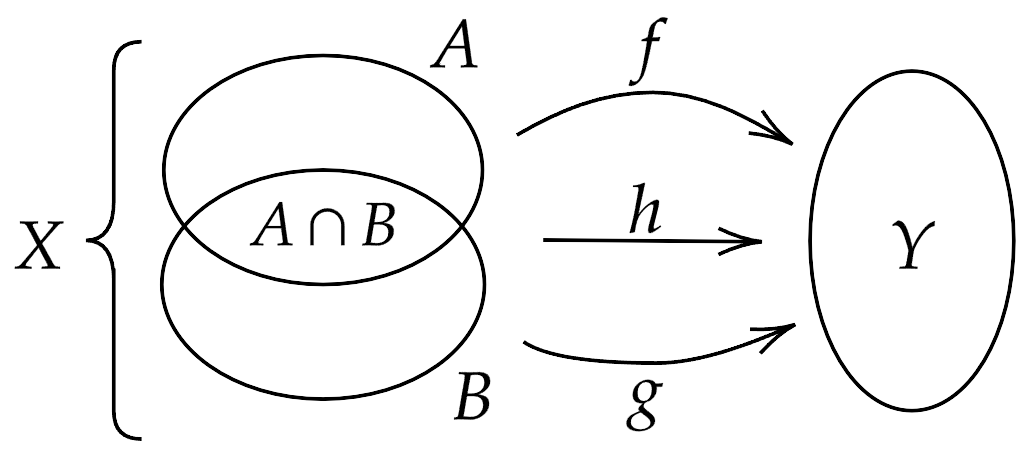
\includegraphics[width=0.4\textwidth]{fig/3.1.png}
    \captionof{figure}{粘贴引理示意图}
\end{figure}
\begin{proof}
    $\forall\,\close C\in Y$，则$f^{-1}(C)$是$A$中的闭集，$g^{-1}(C)$是$B$中的闭集.\par
    且由$x\in h^{-1}(C)\Leftrightarrow h(x)\in C \Leftrightarrow f(x)\in C\text{或} g(x)\in C\Leftrightarrow x\in f^{-1}(C)\text{或} x\in g^{-1}(C)\Leftrightarrow x\in f^{-1}(C)\cup g^{-1}(C)$，可知$h^{-1}(C)=f^{-1}(C)\cup g^{-1}(C)$\par
    根据定义，$\exists\,\close D_1\in X,\st f^{-1}(C)=D_1\cap A$.\par
    同理，$\exists\,\close D_2\in X,\st g^{-1}(C)=D_2\cap B$.\par
    因为$A,B$都是$X$中的闭集，$f^{-1}(C)$和$g^{-1}(C)$都是$X$中的闭集，因此$h^{-1}(C)=f^{-1}(C)\cup g^{-1}(C)$也是$X$中的闭集.\par
    因此$h$是连续的.
\end{proof}
\begin{remark}
    将上述引理中的闭集改为开集，结论同样成立，证明过程类似.
\end{remark}

\section{同胚}

下面介绍一种特殊的连续映射，称为同胚，它是衡量拓扑空间“相似性”的重要工具，其严格定义如下：

\begin{definition}{同胚}
    设 $X,Y$ 是拓扑空间，$f:X\to Y$ 是一个具有逆映射 $f^{-1}:Y\to X$ 的双射.如果 $f$ 和 $f^{-1}$ 都是连续的, 则称 $f$ 是一个\textbf{同胚}.\par
    如果存在一个在 $X$ 和 $Y$ 之间的同胚, 则称 $X$ 和 $Y$ 是\textbf{同胚的}, 记作 $X\cong Y$.
\end{definition}

\begin{remark}
    设 $f:X\stackrel{\cong}{\longrightarrow} Y$，那么 $f$ 是 $X$ 中的点与 $Y$ 中的点之间的一个双射.并且$f$可以诱导$X$ 中的开集与 $Y$ 中的开集之间的一个双射.
    \begin{enumerate}[(i)]
        \item $\forall\, X$ 中的开集$U$, $f(U)$ 是 $Y$ 中的开集.\par
        [$f^{-1}:Y\to X$ 是连续的 $\Rightarrow (f^{-1})^{-1}(U)$ 在 $Y$ 中是开集, 即 $f(U)$ 在 $Y$ 中是开集]
        \item $\forall\, Y$ 中的开集$V$, $f^{-1}(V)$ 是 $X$ 中的开集.\par
        [$f:X\to Y$ 是连续的 $\Rightarrow f^{-1}(V)$ 在 $X$ 中是开集]
    \end{enumerate}
\end{remark}

\begin{proposition}
    关系“$\cong$”是拓扑空间之间的一个等价关系.
    \begin{enumerate}[(i)]
        \item $X\cong X$
        \item $X\cong Y \Rightarrow Y\cong X$
        \item $X\cong Y, Y\cong Z \Rightarrow X\cong Z$
    \end{enumerate}
\end{proposition}

\begin{instance}
    \begin{enumerate}
        \item 取$(-1,1)\subset \mb{E}^1$，则$(-1,1)\cong \mb{E}^1$.\par
        可以构造双射$f:(-1,1)\to\mb{E}^1, x\mapsto \frac{x}{1-|x|}$，$f^{-1}:\mb{E}^1\to(-1,1), y\mapsto \frac{y}{1+|y|}$.

        \item 取$n$维欧氏空间中的单位开球$\mathring{D}^n = \{(x_1,\dots,x_n)\in\mb{E}^n | x_1^2+\dots+x_n^2 < 1\}$. 则$\mathring{D}^n \cong \mb{E}^n$.\par
        同样地，可以构造双射$\setjot[-6]\begin{aligned}[t]
            f:\mathring{D}^n&\to\mb{E}^n \\
            x&\mapsto \frac{x}{1-\|x\|}
        \end{aligned}$，$\setjot[-6]\begin{aligned}[t]
            f^{-1}:\mb{E}^n&\to\mathring{D}^n \\ 
            y&\mapsto \frac{y}{1+\|y\|}
        \end{aligned}$.其中$\|x\|=\sqrt{x_1^2+\dots+x_n^2}$.\par
        当$n=1$时，就是$1$中的情形.
        \item 取$n$维欧氏空间中的开立方体$\mathring{C}^n = \big\{(x_1,\dots,x_n)\in\mb{E}^n \big| |x_i|<1, i=1,\dots,n\big\}$. 则 $\mathring{C}^n \cong \mb{E}^n$.\par
        存在双射：$\setjot[-6]\begin{aligned}[t]
            f:\mathring{C}^n&\to\mb{E}^n \\
            (x_1,\dots,x_n)&\mapsto \left(\frac{x_1}{1-|x_1|},\dots,\frac{x_n}{1-|x_n|}\right)
        \end{aligned}$\quad$\setjot[-6]\begin{aligned}[t]
            f^{-1}:\mb{E}^n&\to\mathring{C}^n \\
            (y_1,\dots,y_n)&\mapsto \left(\frac{y_1}{1+|y_1|},\dots,\frac{y_n}{1+|y_n|}\right)
        \end{aligned}$\par
        其中$\|x\|=\sqrt{x_1^2+\dots+x_n^2}$.\par
        \item 由传递性可知$\mathring{D}^n \cong \mathring{C}^n$，也就是$n$维开球与$n$维开立方体是同胚的.
    \end{enumerate}\par
    \begin{center}
        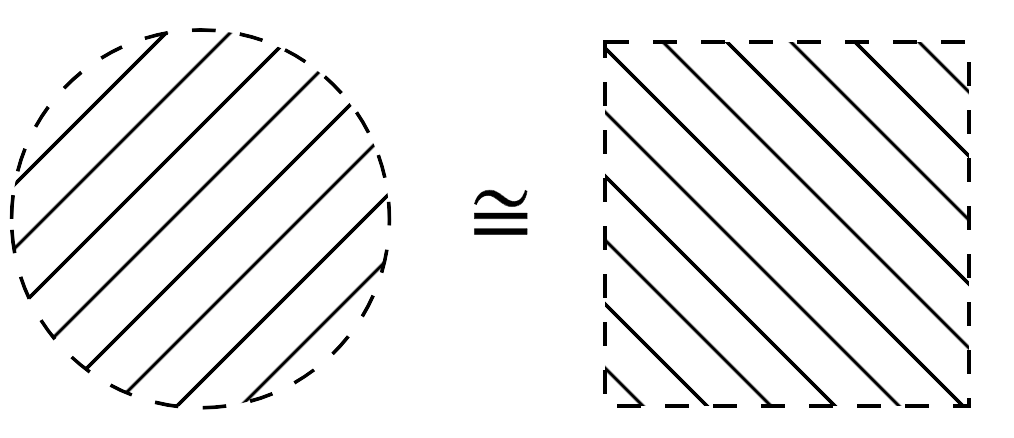
\includegraphics[width=0.3\textwidth]{fig/3.2.png}
        \captionof{figure}{开球与开立方体同胚示意图}
    \end{center}
    \begin{enumerate}
        \setcounter{enumi}{4}
        \item (i)所有的开区间同胚$(a,b)\cong(-\infty,c)\cong(d,+\infty)\cong\mb{E}^1$.\par
        (ii)所有的半开半闭区间同胚$[a,b)\cong[c,d)\cong(-\infty,e]\cong[f,+\infty)$.\par
        (iii)所有的闭区间同胚$[a,b]\cong[c,d]$.
        \item $\mb{E}^n-\{0\} \cong \mb{E}^n-D^n$，其中${D}^n = \{(x_1,\dots,x_n)\in\mb{E}^n | x_1^2+\dots+x_n^2\leq 1\}$.\par
        $\setjot[-4]\begin{aligned}[t]
            f:\mb{E}^n-\{0\}&\to\mb{E}^n-D^n \\
            x&\mapsto x+\frac{x}{\|x\|}
        \end{aligned}$.
        $\setjot[-4]\begin{aligned}[t]
            f^{-1}:\mb{E}^n-D^n&\to\mb{E}^n-\{0\} \\
            y&\mapsto y-\frac{y}{\|y\|}
        \end{aligned}$.

        \item 考虑球面$S^2=\{(x_1,x_2,x_3)\in\mb{E}^3 | x_1^2+x_2^2+x_3^2=1\}$.
        令 $N=(0,0,1)\in S^2$是球面的北极点. 则 $S^2-\{N\}\cong\mb{E}^2$.也就是我们可以把球面上除了北极点之外的点和平面上的点作一一对应.这被称为\bluebf{球极投影}.\par
        构造双射：$\setjot[-4]\begin{aligned}[t]
            f:S^2-\{N\}&\to\mb{E}^2 \\
            (x_1,x_2,x_3)&\mapsto\left(\frac{2x_1}{1-x_3},\frac{2x_2}{1-x_3},-1\right)
        \end{aligned}$.\par
        以及$\setjot[-4]\begin{aligned}[t]
            f^{-1}:\mb{E}^2&\to S^2-\{N\} \\
            (y_1,y_2)&\mapsto\left(\frac{2y_1}{y_1^2+y_2^2+1},\frac{2y_2}{y_1^2+y_2^2+1},\frac{y_1^2+y_2^2-1}{y_1^2+y_2^2+1}\right)
        \end{aligned}$.
    \end{enumerate}\par
    \begin{center}
        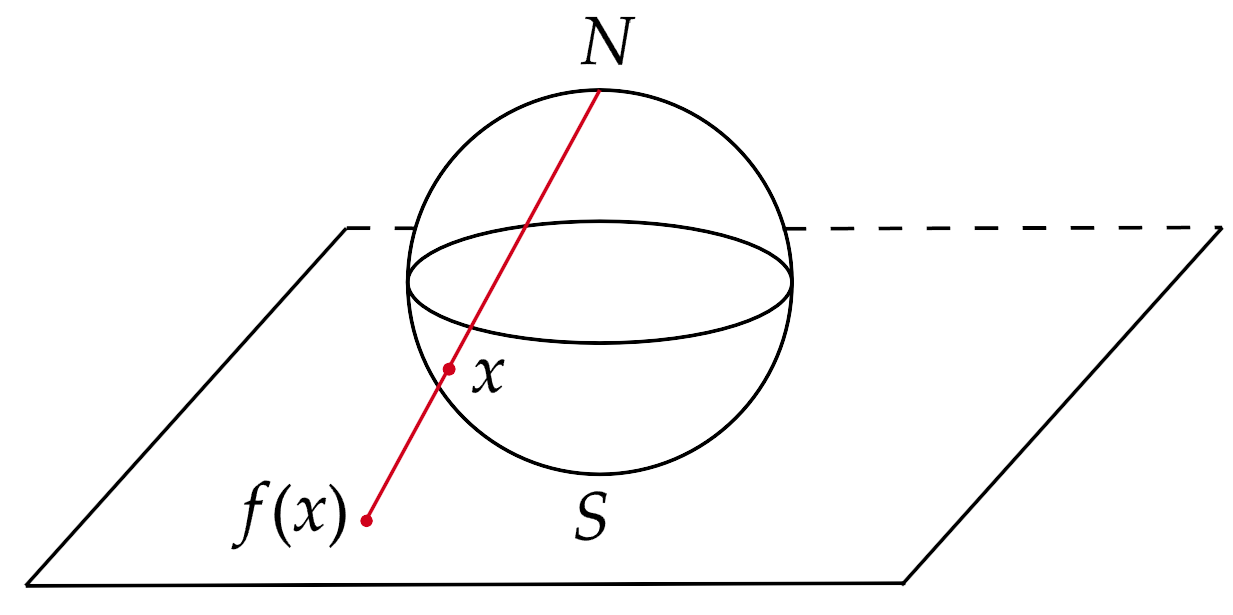
\includegraphics[width=0.4\textwidth]{fig/3.3.png}
        \captionof{figure}{球极投影示意图}
    \end{center}
    \begin{enumerate}
        \setcounter{enumi}{7}
        \item 同样的道理，对于$n+1$维欧氏空间中的超球面$S^n\subset\mb{E}^{n+1}$. $S^n-\{\text{pt}\}\cong\mb{E}^n, n\ge 1$.
    \end{enumerate}
\end{instance}

\begin{definition}{开映射和闭映射}
    映射 $f:X\to Y$ 称为\textbf{开映射} (相应地, \textbf{闭映射})，如果 $f$ 将 $X$ 中的每个开集 (相应地, 闭集) 映射到 $Y$ 中的一个开集 (相应地, 闭集).
\end{definition}
上述概念和连续映射不同. 连续映射要求开集的原像是开集, 而开映射要求开集的像是开集.\par
\begin{remark}
    同胚 $f:X\cong Y$ 既是开映射也是闭映射.\par
\end{remark}

\begin{instance}
    投射 $\setjot[-6]\begin{aligned}[t]
        \pi_1:X\times Y&\to X \\
         (x,y)&\mapsto x
    \end{aligned}$是开映射，因为$\pi_1 \left(\bigcup_\lambda{(U_\lambda\times V_\lambda)}\right)=\bigcup_\lambda{U_\lambda}$.
\end{instance}

\begin{proposition}
    设 $X,Y$ 是拓扑空间. $f:X\to Y$ 是一个同胚 $\Leftrightarrow$ $f$ 是双射、连续的开映射 $\Leftrightarrow$ $f$ 是双射、连续的闭映射.
\end{proposition}
对上述命题，由于同胚包含$f$是连续双射以及$f^{-1}$是连续的，因此我们只需要证明$f^{-1}$连续$\Leftrightarrow f$是开映射.
\begin{proof}
    “$\Rightarrow$” $\forall$ 开集 $U\subset X$, 因为 $f^{-1}:Y\to X$ 是连续的, $(f^{-1})^{-1}(U)$ 在 $Y$ 中是开集, 即 $f(U)$ 在 $Y$ 中是开集. 所以 $f$ 是一个开映射.\par
    “$\Leftarrow$” $\forall$ 开集 $U\subset X$, 因为 $f:X\to Y$ 是开映射, $f(U)=\left(f^{-1}\right)^{-1}(U)$ 在 $Y$ 中是开集. 所以 $f^{-1}:Y\to X$ 是连续的.
\end{proof}

\begin{theorem}
    如果 $f:X\to Y$ 是一个同胚且 $X$ 是Hausdorff空间, 那么 $Y$ 也是Hausdorff空间.
\end{theorem}
\begin{proof}
    $\forall\, y_1,y_2\in Y, y_1\neq y_2$. 则 $f^{-1}(y_1)\neq f^{-1}(y_2)$.\par
    因为 $X$ 是Hausdorff空间, 存在不相交的开集 $U_1, U_2$ 使得 $f^{-1}(y_1)\in U_1, f^{-1}(y_2)\in U_2$.\par
    由于 $f$ 是同胚, $f(U_1)$ 和 $f(U_2)$ 是 $Y$ 中的开集, 且 $y_1\in f(U_1), y_2\in f(U_2)$.
    $f(U_1)\cap f(U_2) = f(U_1\cap U_2) = f(\emptyset) = \emptyset$.
    因此 $Y$ 是Hausdorff空间.
    \begin{center}
        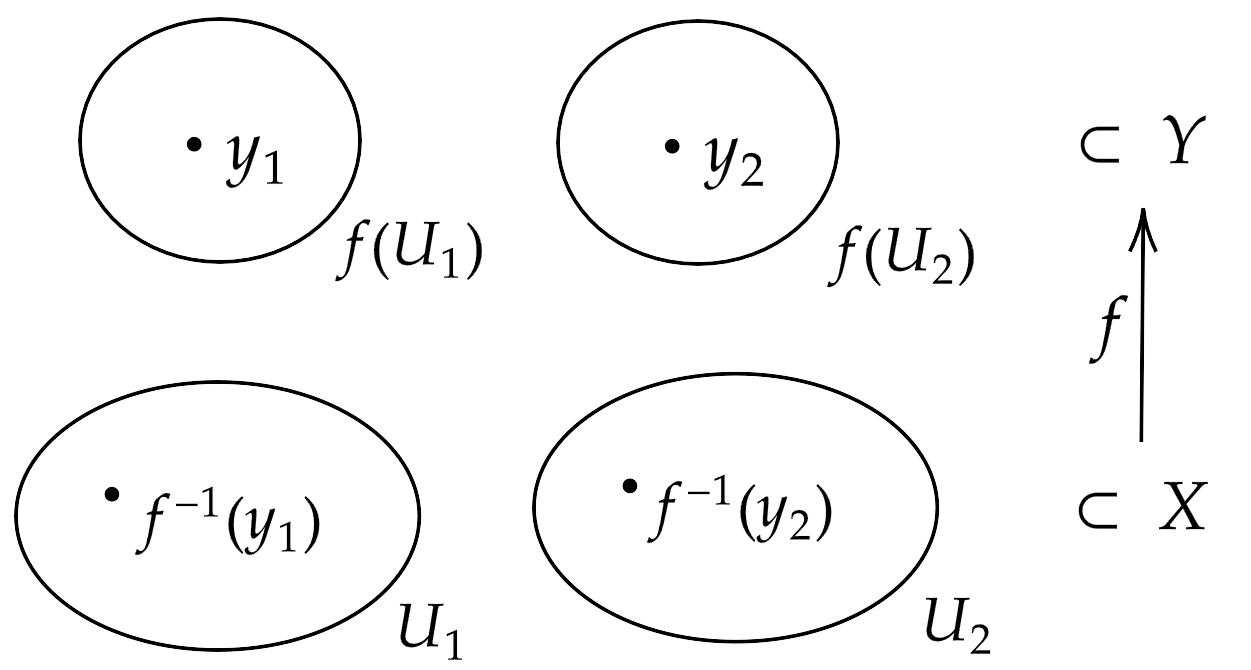
\includegraphics[width=0.5\textwidth]{fig/3.4.png}
        \captionof{figure}{同胚保持Hausdorff性质}
    \end{center}
\end{proof}

\begin{instance}
    $\mb{E}^1\not\cong \mb{R}_{fc}$ (有限补拓扑). 因为 $\mb{E}^1$ 是Hausdorff空间, 而 $\mb{R}_{fc}$ 不是.
\end{instance}

最后我们引入如下的概念：
\begin{definition}{拓扑性质}
    一个拓扑空间的性质, 如果在同胚下保持不变, 则称之为一个\textbf{拓扑性质}.
\end{definition}
因此，一个拓扑空间的Hausdorff性质是一个拓扑性质.\par

\section{嵌入}

\begin{definition}{嵌入}
    设$X,Y$是拓扑空间，则$X$ 在 $Y$ 中的一个\textbf{嵌入}是一个连续映射 $f:X\to Y$, 它将 $X$ 同胚地映射到子空间 $f(X)\subset Y$ 上.
\end{definition}
\begin{figure}[h]
    \centering
    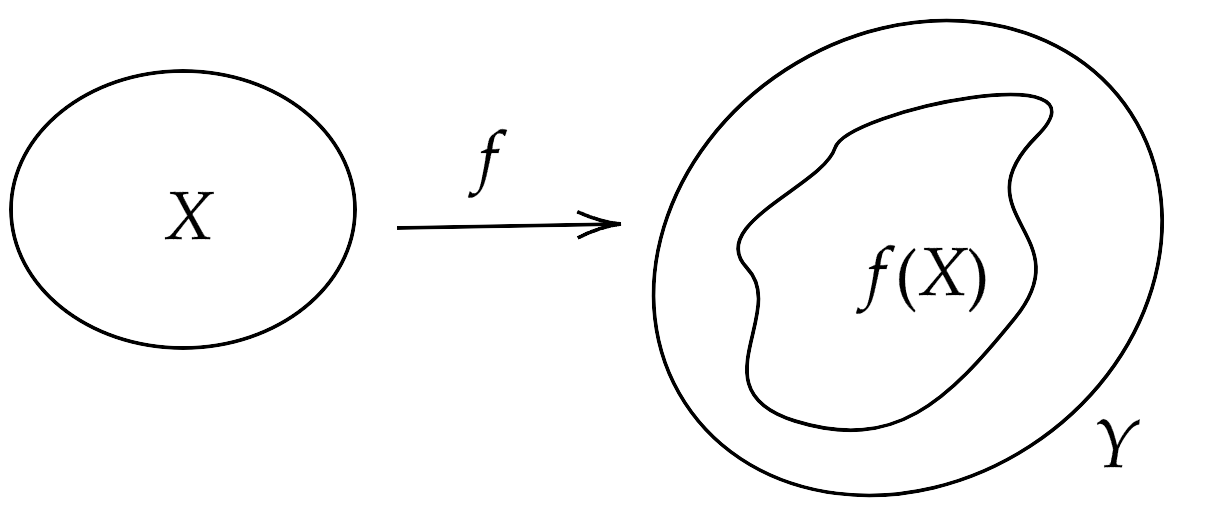
\includegraphics[width=0.5\textwidth]{fig/3.5.png}
    \captionof{figure}{嵌入}
\end{figure}
\begin{remark}
    嵌入是单射.
\end{remark}

\begin{instance}
    在单位圆周$S^1$上，$f:S^1\to\mb{E}^2$ 是一个嵌入.
    \begin{center}
        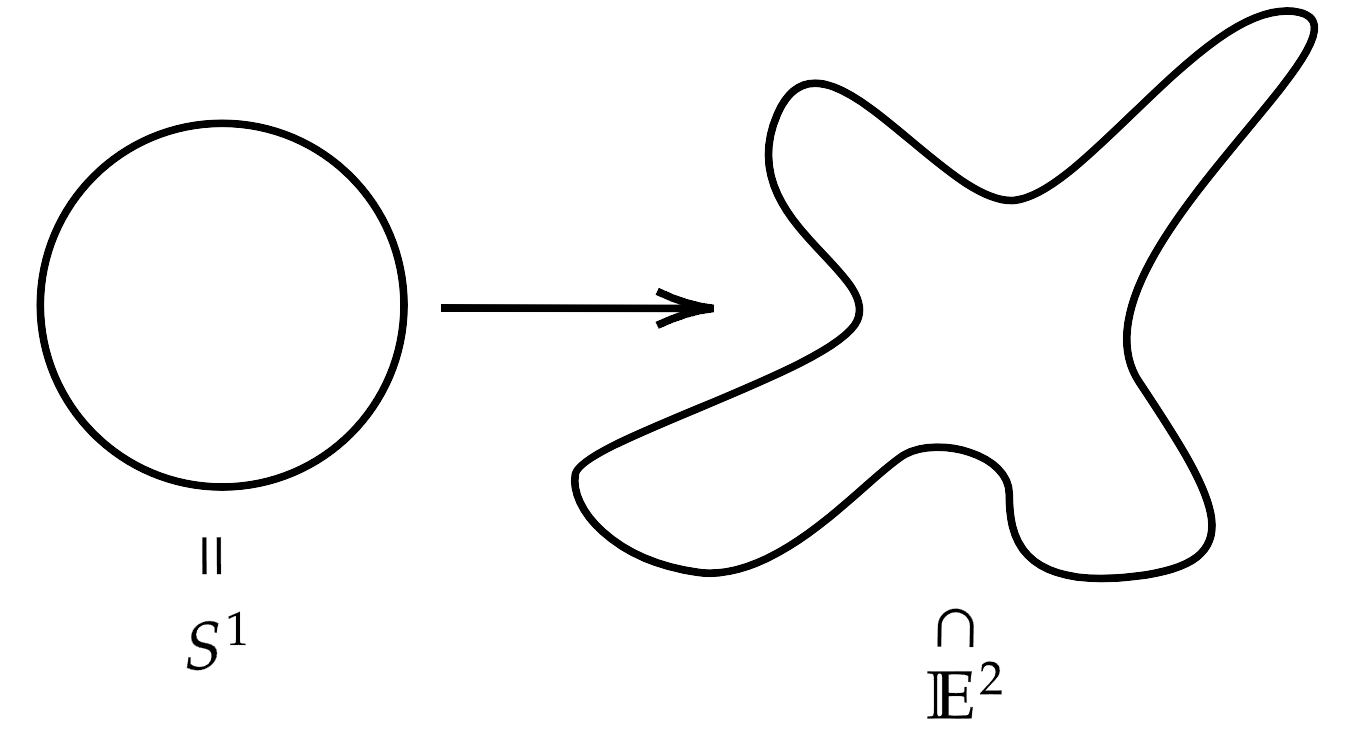
\includegraphics[width=0.5\textwidth]{fig/3.6.png}
        \captionof{figure}{圆的嵌入}
    \end{center}
\end{instance}
\begin{instance}
    下面这个$f:S^1\to\mb{E}^2$的映射不是一个嵌入.其原因在于它将圆上的两个点映射到同一个点上(也就是曲线的交点)，因此不是单射.
    \begin{center}
        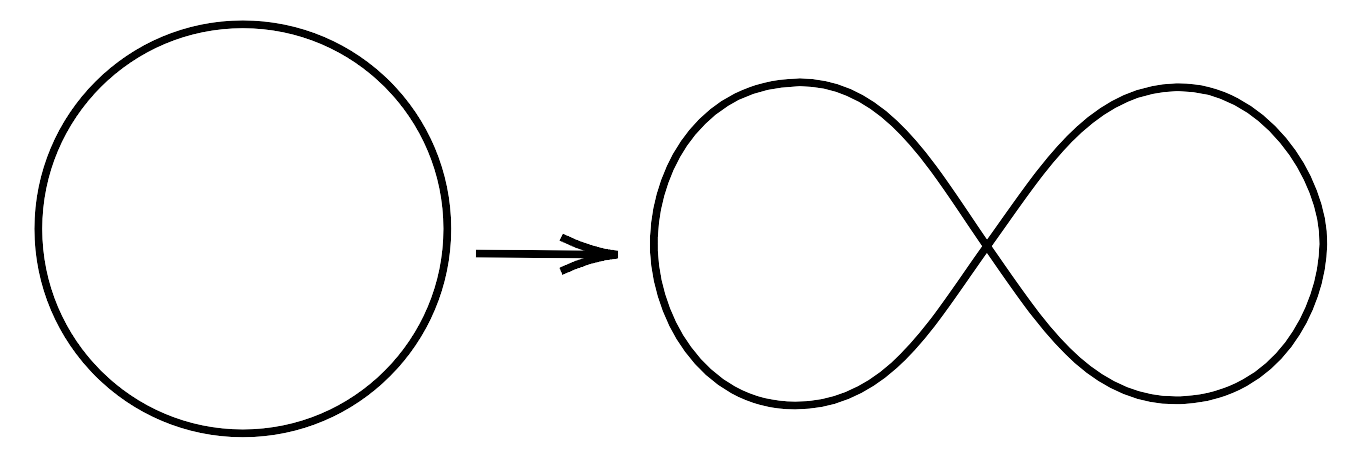
\includegraphics[width=0.5\textwidth]{fig/3.7.png}
        \captionof{figure}{非嵌入的映射}
    \end{center}
\end{instance}
\begin{instance}
    单位圆周到$3$维欧氏空间的映射$f:S^1\to\mb{E}^3$ 是一个嵌入, 称为一个\bluebf{纽结 (Knot)}.
    \begin{center}
        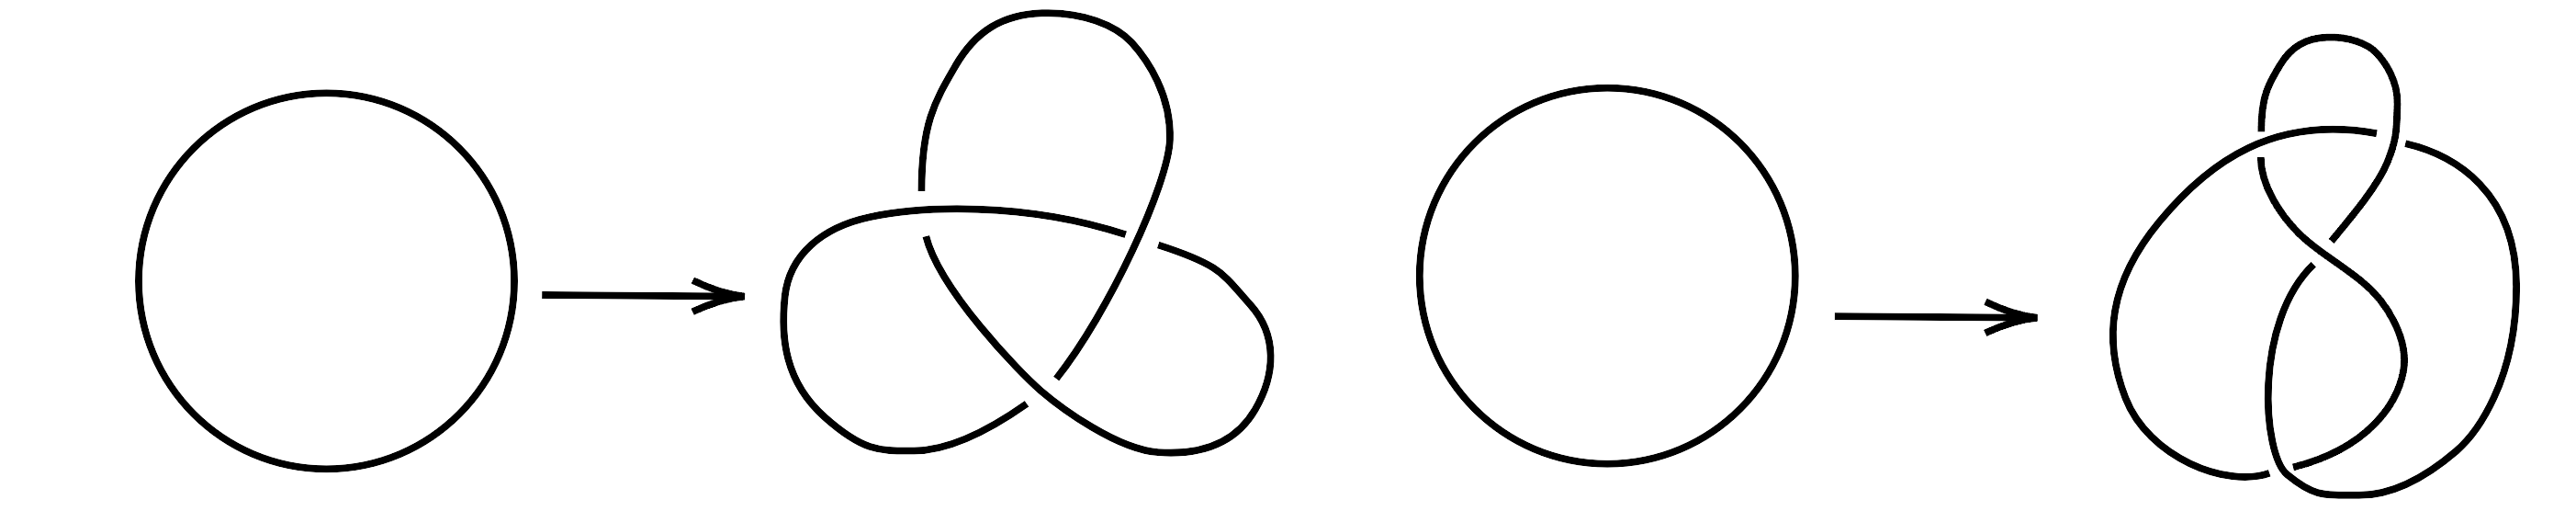
\includegraphics[width=1\textwidth]{fig/3.8.png}
        \captionof{figure}{纽结}
    \end{center}
\end{instance}

关于嵌入，我们也有类似于同胚的快捷的判断方法：
\begin{proposition}
    设$X,Y$是拓扑空间，$f:X\to Y$是一个嵌入$\Leftrightarrow f$是单射、连续的开映射$\Leftrightarrow f$是单射、连续的闭映射.
\end{proposition}


\begin{definition}{同痕}
    设 $f_0, f_1: S^1 \to \mb{E}^3$ 是两个嵌入. 如果存在一个连续映射 $F:S^1\times[0,1]\to\mb{E}^3$, 使得
    $F(x,0)=f_0(x)$, $F(x,1)=f_1(x)$, 并且对$\forall\, t\in[0,1]$, 映射 $f_t=F(\cdot,t):\setjot[-6]\begin{aligned}[t]
        S^1&\to\mb{E}^3\\
        x&\mapsto F(x,t)
    \end{aligned}$ 都是一个嵌入，那么称 $f_0$ 和 $f_1$ 是\textbf{同痕的 (isotopic)}.
\end{definition}
同痕描述了拓扑空间中两个嵌入映射之间的关系.如果两个嵌入映射是同痕的，那么它们之间就可以通过连续的嵌入映射相互转换.

\begin{instance}
    下图中的两个纽结是同痕的.
    \begin{center}
        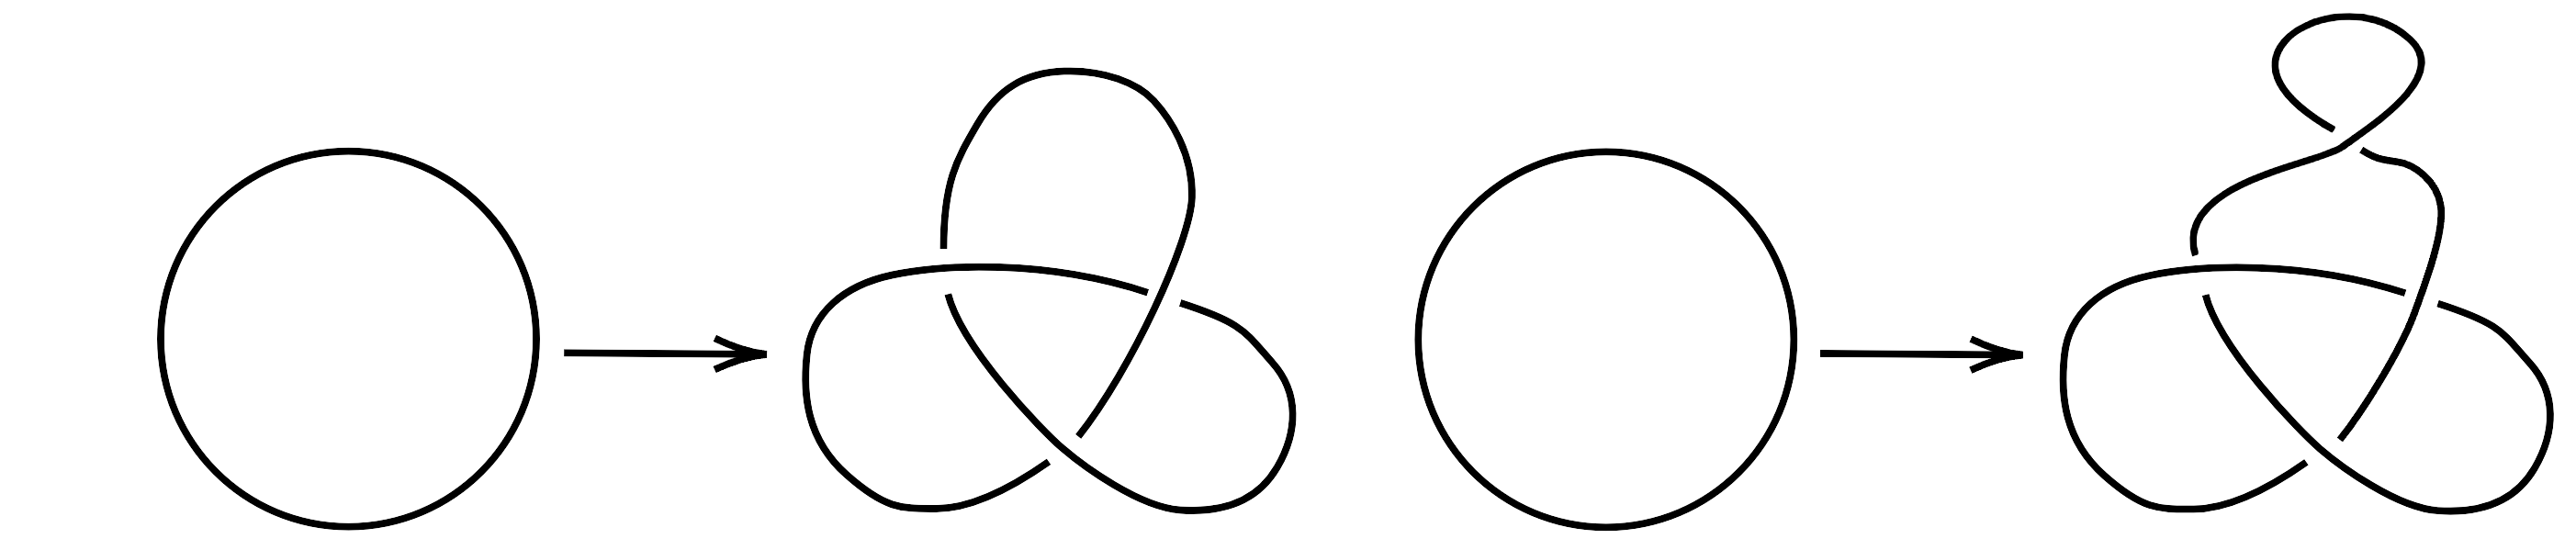
\includegraphics[width=1\textwidth]{fig/3.9.png}
        \captionof{figure}{同痕的纽结}
    \end{center}
\end{instance}

\begin{instance}
    $f:S^1\to T^2$ 的嵌入.
    \begin{center}
        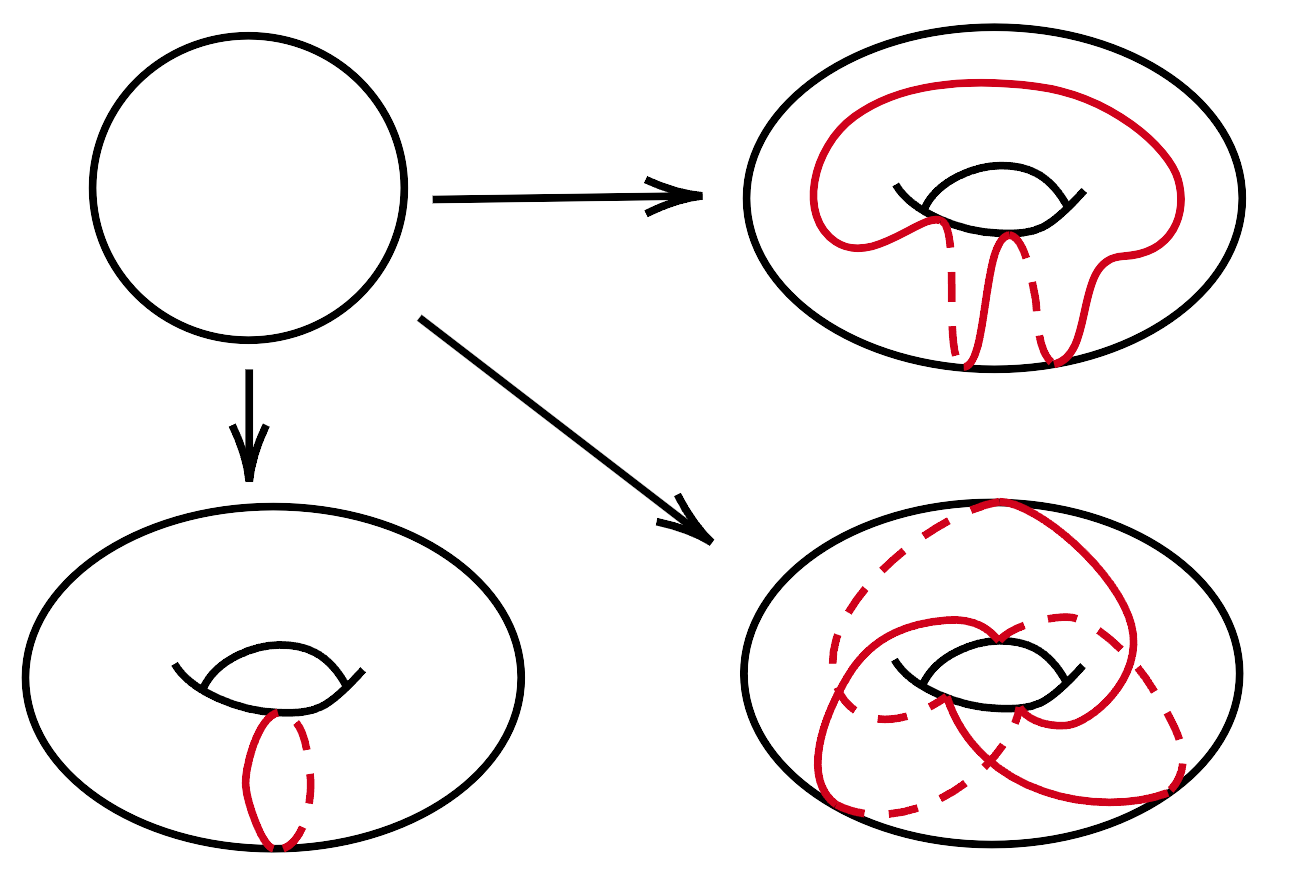
\includegraphics[width=0.5\textwidth]{fig/3.10.png}
        \captionof{figure}{圆环上的嵌入}
    \end{center}
\end{instance}




\chapter{度量空间}

\section{度量和度量拓扑}

\begin{definition}{度量}
    设 $X$ 是一个集合.如果$X$上的函数 $\setjot[-4]\begin{aligned}[t]
        d:X\times X&\to \mb{R}\\
        (x,y) &\mapsto d(x,y)
    \end{aligned}$满足:
    \begin{enumerate}[(i)]
        \item $d(x,y)\ge 0$，等号成立 $\Leftrightarrow x=y$.
        \item $d(x,y)=d(y,x)$.(对称性)
        \item $d(x,y)+d(y,z)\geq d(x,z)$. (三角不等式)
    \end{enumerate}
    则称$d$是$X$的一个\textbf{度量}，$d(x,y)$称为$x$和$y$之间的\textbf{距离}，$(X,d)$ 称为一个\textbf{度量空间}.
\end{definition}

\begin{instance}
    \begin{enumerate}
        \item 在$\mb{R}^n$中，$x=(x_1,\dots,x_n), y=(y_1,\dots,y_n)$.则$d(x,y)=\sqrt{(x_1-y_1)^2+\dots+(x_n-y_n)^2}$是一个度量，是最常见的欧式距离.
        \item $\mb{R}^n$, $d_1(x,y)=|x_1-y_1|+\dots+|x_n-y_n|$是一个度量，称为\bluebf{曼哈顿距离}.
    \end{enumerate}
\end{instance}

在度量空间上，可以自然地定义如下的拓扑：
\begin{definition}{度量拓扑}
    $\forall\, x\in (X,d)$, 开球 $B(x,\varepsilon)=\{y\in X | d(x,y)<\varepsilon\}$.则$\mcal{B}=\{B(x,\varepsilon)|x\in X, \varepsilon>0\}$ 是 $X$ 上的一个拓扑基.由这个拓扑基生成的拓扑称为由度量 $d$ \textbf{诱导的度量拓扑}.
\end{definition}

\begin{proof}
    只需证明$\mcal{B}$是一个拓扑基.\par
    \begin{minipage}[t]{0.725\textwidth}
    (a) $\forall\, x\in X$, $x\in B(x,\varepsilon)$, 所以 $X=\bigcup_{x\in X}B(x,\varepsilon)$.\par
    (b) 设 $x\in B(x_1,\varepsilon_1)\cap B(x_2,\varepsilon_2)$，则 $d(x,x_1)<\varepsilon_1$ 且 $d(x,x_2)<\varepsilon_2$.\par    
    可以取$0<\varepsilon < \min\{\varepsilon_1-d(x,x_1), \varepsilon_2-d(x,x_2)\}$，那么$x\in B(x,\varepsilon)\subset B(x_1,\varepsilon_1)\cap B(x_2,\varepsilon_2)$.\par
    因为$\forall\, y\in B(x,\varepsilon)$，由三角不等式可知$d(y,x_1)\leq d(y,x)+d(x,x_1) < \varepsilon+d(x,x_1) < \varepsilon_1-d(x,x_1)+d(x,x_1)=\varepsilon_1$，所以 $y\in B(x_1,\varepsilon_1)$.同理 $y\in B(x_2,\varepsilon_2)$.\par
    因此$y\in B(x_1,\varepsilon_1)\cap B(x_2,\varepsilon_2)$，故$B(x,\varepsilon)\subset B(x_1,\varepsilon_1)\cap B(x_2,\varepsilon_2)$
    \end{minipage}
    \begin{minipage}[t]{0.21\textwidth}
        \vspace{-2em}
        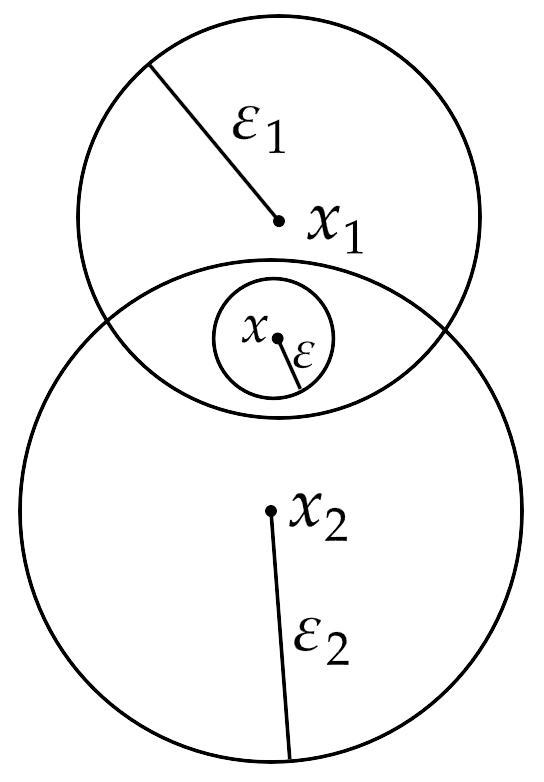
\includegraphics[width=1\textwidth]{fig/4.1.png}
        \captionof{figure}{}
    \end{minipage}
\end{proof}

上述定义表示度量空间是一个比拓扑空间更强的条件，所有的度量空间都是拓扑空间.除此之外，由度量诱导的拓扑也具有更好的性质：
\begin{proposition}
    每个度量空间都是Hausdorff空间.
\end{proposition}
\begin{proof}
    假设 $(X,d)$ 是一个度量空间, $x_1,x_2$ 是 $X$ 中两个不同的点.则$d(x_1,x_2)>0$.\par
    令 $\varepsilon = \frac{1}{3}d(x_1,x_2)$，则$B(x_1,\varepsilon)$ 和 $B(x_2,\varepsilon)$ 分别是 $x_1,x_2$ 的邻域.\par
    下证$B(x_1,\varepsilon)\cap B(x_2,\varepsilon)=\emptyset$.\par
    (反证)假设$y\in B(x_1,\varepsilon)\cap B(x_2,\varepsilon)$，则$d(x_1,x_2)\leq d(x_1,y)+d(y,x_2) < 2\varepsilon = \frac{2}{3}d(x_1,x_2)$.矛盾!
\end{proof}
\begin{corollary}
    度量空间中的每个单点集都是闭集.
\end{corollary}

\begin{instance}
    若$X\neq\varnothing$，则$d(x,y)=\begin{cases} 0, & \text{if } x=y \\ 1, & \text{if } x\neq y \end{cases}$是一个度量，称为\bluebf{离散度量}.它诱导的$X$上的开球形如$B(x,\varepsilon) = \begin{cases} \{x\}, & \text{if } \varepsilon\leq 1 \\ X, & \text{if } \varepsilon > 1 \end{cases}$.则拓扑基$\mcal{B}=\{B(x,\varepsilon)|x\in X, \varepsilon>0\}$生成了$X$ 上的离散拓扑.
\end{instance}



\begin{definition}{可度量化}
    $X$ 是一个拓扑空间.如果在 $X$ 上存在一个度量 $d$ 诱导了 $X$ 上的拓扑，则称$X$ 是\textbf{可度量化的}.
\end{definition}

\begin{instance}
    \begin{enumerate}
        \item 离散拓扑是可度量化的.
        \item 如果 $X$ 不是Hausdorff空间, 那么 $X$ 是不可度量化的. 例如, $\mb{R}_{fc}$是不可度量化的.
    \end{enumerate}
\end{instance}
